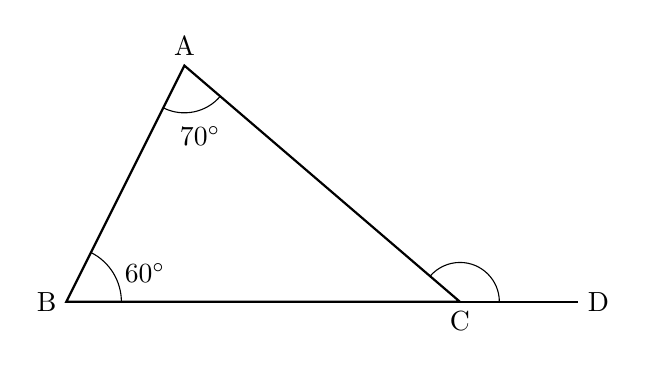
\begin{tikzpicture}

% Define the coordinates of the triangle vertices
\coordinate (B) at (0,0);
\coordinate (C) at (5,0);
\coordinate (A) at (1.5,3);

% Define point D on the extension of BC
\coordinate (D) at (6.5,0);

% Draw the triangle sides
\draw[thick] (A) -- (B) -- (C) -- cycle;

% Draw the extended line CD
\draw[thick] (C) -- (D);

% Draw the angle arc at vertex A (70 degrees)
\draw (A) ++(-40:0.6) arc (-40:-117:0.6);

% Draw the angle arc at vertex B (60 degrees)
\draw (B) ++(0:0.7) arc (0:63:0.7);

% Draw the exterior angle arc at vertex C
\draw (C) ++(0:0.5) arc (0:140:0.5);

% Label the vertices
\node[above] at (A) {A};
\node[left] at (B) {B};
\node[below] at (C) {C};
\node[right] at (D) {D};

% Label the angle at A (70 degrees)
\node at (1.7,2.1) {$70^{\circ}$};

% Label the angle at B (60 degrees)
\node at (1,0.37) {$60^{\circ}$};

\end{tikzpicture}